\documentclass{article}

\author{Pedro Henrique Limeira da Cruz}
\title{EM461 - Mecânica dos Fluidos I}

\usepackage[margin=0.8in]{geometry}
\usepackage{indentfirst}
\usepackage{fancyhdr}
\usepackage{tcolorbox}
\usepackage{graphicx}
\usepackage{amsmath}
\usepackage{amssymb}
\usepackage{tabularx}
\usepackage{subcaption}
\usepackage{float}
\usepackage{array}

% Create a new command to be used in the align environment in multiple line equations do only the last equation is numbered  
\newcommand{\n}{\nonumber \\ }
\makeatletter
\let\inserttitle\@title
\makeatother
% Set the style of the page 
\pagestyle{fancy}
\fancyhf{}
\rhead{Pedro Henrique L. da Cruz}
\lhead{\inserttitle}
\rfoot{Page \thepage}

\usepackage{hyperref}
\hypersetup{
    colorlinks=true,
    linkcolor=black,
    filecolor=magenta,
    urlcolor=cyan,
}

\renewcommand\tabularxcolumn[1]{m{#1}}%


% Begin the Document 
\begin{document}

    \maketitle
    \thispagestyle{empty}

    % Add the image inside a figure in as the first page
    \begin{figure}[h]
        \begin{center}
            
\includegraphics[scale = 0.15]{/Users/pedrocruz/Documents/UNICAMP/ES101/ES101 - Robotic Arm/img/unicamp.png}
        \end{center}
    \end{figure}

    % Change to the Next page 
    \newpage
    \tableofcontents
    \newpage

    \section{Estática dos Fluidos}
        Antes de começarmos nossos estudos sobre a mecânica dos fluidos em movimento, iremos revisar (ou para alguns introduzir) a estática de fluidos. 

        \subsection{Equação Base - Estática de Fluidos}
            A equação mais básica da estática de fluidos é aquela que modela o campo de pressão em um fluido estático. A partir das experiências do dia-a-dia podemos verificar o principal aspecto
            sobre a pressão em uma coluna de fluido estático: 

            \begin{center}
                \textbf{A pressão Aumenta com a Profundidade}
            \end{center}

            A partir disso, e com a intenção de modelarmos matematicamente o sistema, fazemos a análise mais básica de mecânica estática, a lei de Newton. Para esse caso, entretanto, como estamos
            falando de um fluido e não de um corpo concentrado, iremos aplicar a lei de newton em um cenário diferencial, para lidarmos com pequenas massas (ou pequenos volumes) do fluido, como mostra a equação \ref{eq:newton_diff_base}:
            \begin{align}
                d\vec{F}_{resultante}= \vec a dm \label{eq:newton_diff_base}
            \end{align}

            A partir disso, como temos nossa lei de newton básica (mas agora aplicada para o problemas diferencial de fluidos), podemos prosseguir e identificar as forças envolvidas.

            A primeira força de campo que iremos ver e que atua nos problemas de estática de fluidos é a força oriunda da \emph{gravidade}, quando analisamos um pequeno volume diferencial do fluido, dada por:
            \begin{align}
                d\vec{F}_B = \vec{g}\rho d \forall \label{eq:forca_peso}
            \end{align}

            Onde:
            \begin{itemize}
                \item $\rho$: Massa específica. Para problemas que estaremos analisando é constante em função tanto do tempo quanto posição.
                \item $\forall$: Volume do elemento, dada em coordenadas cartesianas tal que $d\forall = dx \ dy \ dz$
                \item $g$: Aceleração da gravidade.
            \end{itemize}

            A segunda força que iremos analisar agora é a \textbf{única força de superfície} presente, tendo em vista que estamos abordado a estática de fluidos e, por conseguinte, não há a presença
            de tensão de cisalhamento, é a \textbf{força de pressão de superfície} $p = p(x, y, z)$ (um vetor com três componentes), que varia conforme a posição dentro do fluido. Podemos entender essa pressão de superfície como sendo a 
            \textbf{Pressão exercida pela coluna de fluido ao redor do volume diferencial sendo estudado}.

            A partir disso, temos a Lei de Newton que governa o problema diferencial do fluido (dado pela equação \ref{eq:newton_diff_base}) e temos que as únicas forças que atua no nosso problema são a
            força de pressão $p(x, y, z)$ e a força peso do volume diferencial sob análise. Como estamos lidando com um problema de estática a somatória de todas as forças precisa ser zero, temos:

            \begin{align}
                d\vec{F} = (-\nabla p + \rho \vec{g}) d\forall \Rightarrow \frac{d\vec{F}}{d\forall} = -\nabla p + \rho \vec g \label{eq:newton_estatica_de_fluidos}
            \end{align}

            Onde temos então a equação final \ref{eq:newton_estatica_de_fluidos}, que representa a força resultante por unidade de volume, que ao igualarmos a zero resulta em:

            \begin{align}
                -\nabla p &+ \rho \vec g = 0\label{eq:newton_resultante_estatica_de_fluidos}
            \end{align}

            Onde:
            \begin{itemize}
                \item $-\nabla p$: Força de pressão resultante por unidade de volume em um ponto. Representado pelo vetor gradiente com uma componente $x$ uma $y$ e uma $z$
                \item $\rho \vec g$: Força de campo (gravitacional) por unidade de volume em um ponto
            \end{itemize}

        \subsection{Variação de Pressão em um Fluido Estático}
            A seção anterior foi de suma importância por introduzir a modelagem amtemática básica para a estática de fluidos, com a equação \ref{eq:newton_resultante_estatica_de_fluidos}. A partir
            disso, podemos dissecar tal equação e relacionarmos o que sabemos na prática (que a pressão aumenta com a profundidade) com a modelagem.

            Para tal, precisamos primeiro considerar que estamos lidando com um \textbf{líquido incompressível}, de tal forma que $\rho=const$ e também que a gravidade é uma constante e aponta na
            direção $z$ somente. A partir disso, precisamos analisar a equação \ref{eq:newton_resultante_estatica_de_fluidos} somente no eixo $z$ , resultando em:

            \begin{align}
                -\nabla p + \rho \vec g &= 0 \n
                -\frac{\partial p}{\partial z} + \rho (-g_z) &= 0 \n
                -\frac{dp}{d z} + \rho (-g_z) &= 0 \label{eq:diff_inicial_pressao} \\
                dp &= +\rho g_z dz \n
                \int^p_{p_0} dp &= \int^z_{z_0} \rho g_z dz \n
                p - p_0 &= \rho g_z (z- z_0) \n 
                \Delta p &= \rho g h  \label{eq:final_delta_p_estatica_de_fluidos}
            \end{align}

            É importante ressaltar que, a equação \ref{eq:final_delta_p_estatica_de_fluidos} só é valida para:
            \begin{itemize}
                \item Fluido Estático
                \item A gravidade é a única força de campo
                \item O eixo $z$ é vertical voltado para cima
            \end{itemize}

            Além disso, a equação \ref{eq:diff_inicial_pressao} é importante para os casos em que o fluido não é incompressível (e por conseguinte a massa específica $\rho$ pode variar com a pressão
            $p$). Para esses casos, devemos partir nossas contas dessa equação e fazer a integral para o devido $\rho = f(p)$, como é nos casos dos gases ideais. Importante ressaltar que o sinal da
            gravidade é negativo pois o eixo $z$ é positivo para cima, \textbf{se o eixo $z$ for positivo para baixo o sinal da gravidade na equação \ref{eq:diff_inicial_pressao} seria positivo}.


            \newpage

        \subsection{Variação de Pressão Em um Gás Ideal}
            Como dito na parte anterior, há casos que lidaremos com fluidos compressíveis, sendo o mais notório deles os chamados \textbf{gases ideais}, onde:
            \begin{align}
                p &= \rho RT \therefore \rho = \frac{P}{RT} \label{eq:gases_ideais}
            \end{align}

            Onde: 
            \begin{itemize}
                \item $T$: Temperatura em Kelvin
                \item $P$: Pressão
                \item $\rho$: Massa Específica
                \item $R$: Constante universal dos gases (tabelada)
            \end{itemize}

            A partir da equação \ref{eq:gases_ideais}, e da equação \ref{eq:diff_inicial_pressao}, somos capazes de determinar uma expressão para a pressão em um gás ideal:
            \begin{align}
                dp &= - \rho g dz \n
                dp &= - \frac{p}{RT} g dz \n
                \frac{1}{p} dp &= -\frac{1}{RT} g dz \n
                \int^p_{p_0}\frac{1}{p} dp &= -\int^z_{z_0}\frac{1}{RT} g dz \n
                \ln{(p/p_0)} &= -\frac{g}{RT} (z - z_0)
            \end{align}

        \newpage

        \subsection{One Pager - Estática de Fluidos}

        \begin{table}[h]\tiny
            \begin{tabularx}{\textwidth}{|l|c|X|}\hline
                \textbf{Uso} & \textbf{Equação} & \textbf{Descrição} \\ \hline 

                \rule{0pt}{7ex}Estática de Fluidos - Geral & $d\vec{F} = \vec{a} dm$ & A segunda Lei de Newton em um formato infinitesimal, base para a análise de forças em Estática dos Fluidos. \\[4ex] \hline 
                \rule{0pt}{7ex}Estática de Fluidos - Geral & $- \nabla p + \rho \vec g = 0$ & A aplicação da segunda lei para um volume infinitesimal de um fluido estático apensa sob pressão e gravidade. OBS: $\nabla p$ representa o vetor
                gradiente nas três direções da pressão. \\ [4ex]\hline

                \rule{0pt}{7ex}Variação de Pressão - Fluido Estático & $dp/dz = -\rho g_z \Rightarrow dp = -\rho g_z dz$ & Aplicação específica da fórmula do volume apensa sob pressão, e gravidade somente no eixo
                $y$, base para problemas para calcular variação de pressão a depender de $z$ (especialmente se $\rho$ depender de $z$ ou de $p$ como no exemplo de gases ideais) \\ [4ex]\hline 

                \rule{0pt}{7ex}Variação de Pressão - Fluido Estático & $\Delta p = \rho g h$ & Variação de pressão para fluidos incompressíveis, estáticos. \\ [4ex]\hline

                \rule{0pt}{7ex}Variação de Pressão - Gás Ideal & $p = \rho RT \Rightarrow \rho = p/RT$ & Fórmula que relaciona pressão e massa específica $\rho$ dos gases ideais. \\ [4ex]\hline

                \rule{0pt}{7ex}Variação de Pressão - Gás Ideal & $\ln{(p/p_0)} = -(g/RT)(z - z_0)$ & Fórmula para variação da pressão em gasses ideais, oriundo da integração da equação diferencial geral de variação
                pressão, em conjunto com a equação que expressa $\rho$ em função de $p$ para gases ideais acima. \\ [4ex]\hline

            \end{tabularx}
        \end{table}
        \newpage

    \section{Conceitos Fundamentais Dinâmica dos Fluidos} 
        Agora que revemos os conceitos mais básicos de Estática dos Fluidos, iremos então explorar os principais conceitos de Dinâmica dos Fluidos, sendo o primeiro deles a ideia de 
        campo de velocidade.
        
        \subsection{Campo de Velocidade}
            Algo muito importante de internalizarmos entes de falarmos sobre a velocidade de um líquido é que ele não é uma partícula, mas sim um conjunto "contínuo" de partículas, por isso chamamos
            um fluido de um "contínuo". Como resultado direto disso, temos que a velocidade de um certo volume de fluido pode depender não somente do tempo (como estamos mais acostumados com corpos
            rígidos), mas também pode depender da posição que está sendo analisada dentro de tal fluido, \emph{i.e} a velocidade é um função da posição da partícula de análise como também do tempo:
            \begin{align}
                \vec V = \vec V (x, y, z, t) = u \hat i + v \hat j + w \hat k \label{eq:campo_velocidade}
            \end{align}

            A partir disso, podemos agrupar os diferentes tipo de escoamento de fluidos em relação a:
            \begin{itemize}
                \item \textbf{Dimensões de Escoamento}:
                    \subitem $\hookrightarrow$ \underline{Escoamento Uni-Dimensional}: O campo de velocidade, no que tange posição, muda em relação a somente uma coordenada.
                    \subitem $\hookrightarrow$ \underline{Escoamento Bi-Dimensional}: O campo de velocidade, no que tange posição, muda em relação a  duas coordenadas.
                    \subitem $\hookrightarrow$ \underline{Escoamento Tri-Dimensional}: O campo de velocidade, no que tange posição, muda em relação a três coordenadas.
                \item \textbf{Variação no Tempo}:
                    \subitem $\hookrightarrow$\underline{Regime Permanente}: A velocidade nem a massa específica variam com o tempo.
                    \subitem $\hookrightarrow$\underline{Regime Transiente}: As propriedades do fluido podem variar em relação ao tempo.
            \end{itemize}

        \subsection{Linhas de Caracterização}
            Para estudarmos o comportamento de um fluido, principalmente da sua interação com outros corpos e superfícies, nós usamos diferentes técnicas, chamadas de linhas de caracterização, sendo
            elas:
            \begin{itemize}
                \item \textbf{Linhas de Tempo}: Análise de Várias partículas adjacentes, em um determinado instante. Obtida via experimento.
                \item \textbf{Linhas de Trajetória}: Análise do caminho traçado por uma partícula em movimento. Obtida via experimento.
                \item \textbf{Linhas de Emissão}: Linha que traça todos os caminhos que particulas que passaram por um determinado ponto no espaço. Obtida via experimento.
                \item \textbf{Linhas de Corrente}: Linhas tangente à direção e velocidade de escoamento em cada ponto do campo. Obtida Matematicamente.
            \end{itemize}

            Sendo que é importante ressaltar que para regime permanente, todas coincidem.

            A que mais vamos ver, por ser obtida matematicamente, é a linha de corrente, que é dada por:
            \begin{align}
                \frac{dy}{dx} \big{)}_{linha \ de \ corrente} = \frac{v}{u}, \ \ \begin{cases}
                    v = v_y \\ 
                    u = v_x
                \end{cases}
            \end{align}

            A partir disso somos capazes de isolar $dx$ com tudo que depende de $x$, e $dy$ com tudo que depende de $y$ e integrar para acharmos uma equação que depende de $x,y$ para a linha de
            corrente.
            
        \subsection{Tensão de Cisalhamento}

            \begin{figure}[H]
                \begin{subfigure}{0.5\textwidth}
                    \centering
                    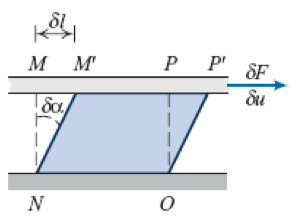
\includegraphics[width=.6\linewidth]{imgs/tens_cisa.png}
                    \caption{Modelagem da Tensão de Cisalhamento}\label{img:tens_cis}
                \end{subfigure}% Really important to have this comment here and no black line
            \begin{subfigure}{.5\textwidth}
                \centering
                    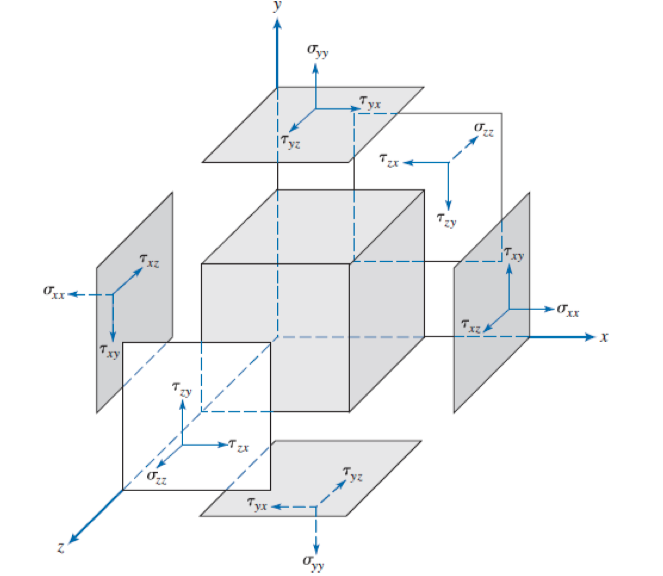
\includegraphics[width=.6\linewidth]{imgs/conv_tens.png}
                    \caption{Convenção de Sinais de Tensão}\label{img:conv_sinais}
                \end{subfigure}
                \caption[]{Modelos para Tensão}
            \end{figure}

            A tensão de cisalhamento é uma tensão oriunda da movimentação relativa entre as faces externas de um fluido. Tal tensão é de suma importância pois, juntamente com a \textbf{condição de não
            escorregamento} (\emph{i.e} que o fluido, no ponto de contato com uma superfície, tem a mesma velocidade que tal superfície) nos possibilita calcular a força de resistência que o fluido
            faz ao deslocamento. 
            Em primeiro lugar, a tensão de cisalhamento é dada por:
            \begin{align}
                \tau_{yx} = \mu \frac{d}{dy} u, \begin{cases}
                    \mu = Viscosidade \\ 
                    u = Velocidade \ no \ eixo \ x
                \end{cases}
            \end{align}

            A partir disso, sabemos que força nada mais é que:
            \begin{align}
                F_{reaction} = \tau_{yx} \cdot A, \ \ A= Contact \ Area
            \end{align}


            Algo importante de elaborarmos é a convenção de sinais para a tensão (e por conseguinte a força de reação). As tensões em um fluido seguem a convenção da imagem \ref{img:conv_sinais}. Isso
            implica, se estamos observando a tensão da superfície superior do fluido, e ela é positiva, temos que ela aponta para a direita, já se estamos observando a tensão da superfície inferior
            do fluido  e é positiva, temos que ela aponta para a esquerda.

            \newpage
        \subsection{One Pager - Conceitos Fundamentais}

            \subsubsection*{Principais Fórmulas}

                \begin{table}[h]\tiny
                    \begin{tabularx}{\textwidth}{|l|c|X|}\hline
                        \textbf{Nome} & \textbf{Equação} & \textbf{Descrição} \\ \hline 

                        \rule{0pt}{10ex} Linha de Corrente & \begin{minipage}{0.5\textwidth}
                                    $$\frac{dy}{dx} \big{)}_{linha \ de \ corrente} = \frac{v}{u}, \ \ \begin{cases}
                                        v = v_y \\ 
                                        u = v_x
                                    \end{cases}$$
                            \end{minipage}&  Calculo da linha de corrente, que é tangente a velocidade em um ponto $x,y$. Podemos separar o que tem $x$ e $dx$ em um lado, $y$ e $dy$ do outro e integrar para achar
                            uma função que depende de $xy$ \\[5ex] \hline

                        \rule{0pt}{8ex} Tensão de Cisalhamento & 
                                    \begin{minipage}{0.5 \textwidth}
                                    $$\tau_{yx} = \mu \frac{d}{dy} u, \begin{cases}
                                        \mu = Viscosidade \\ 
                                        u = Velocidade \ no \ eixo \ x
                                    \end{cases}$$
                                \end{minipage}
                                    
                            & Calculo da Tensão de cisalhamento, o resultado segue a convenção de sinais da imagem \ref{img:conv_sinais}. \\[5ex] \hline

                        \rule{0pt}{8ex} Força de Resistência & 
                                \begin{minipage}{0.5 \textwidth}
                                    $$F_{reaction} = \tau_{yx} \cdot A, \ \ A= Contact \ Area$$
                                \end{minipage}
                            & Calculo da força de resistência ao movimento relativo entre duas placas com líquido no meio. \\[5ex] \hline
            \end{tabularx}

            $\\$
            $\\$

            \subsubsection*{Principais Conceitos}
                $\\$

                \begin{minipage}[c]{0.6 \textwidth}\tiny
                    \begin{itemize}
                        \item \textbf{Dimensões de Escoamento}:
                            \subitem $\hookrightarrow$ \underline{ Uni-Dimensional}: A velocidade muda em relação a somente uma coordenada.
                            \subitem $\hookrightarrow$ \underline{ Bi-Dimensional}: A velocidade muda em relação a  duas coordenadas.
                            \subitem $\hookrightarrow$ \underline{ Tri-Dimensional}: A velocidade muda em relação a três coordenadas.
                        \item \textbf{Variação no Tempo}:
                            \subitem $\hookrightarrow$\underline{Regime Permanente}: A velocidade nem a massa específica variam com o tempo.
                            \subitem $\hookrightarrow$\underline{Regime Transiente}: As propriedades do fluido podem variar em relação ao tempo.
                        \item \textbf{Princípio de Não Escorregamento}:O fluido, no ponto de contato com uma superfície, tem a mesma velocidade que tal superfície
                    \end{itemize}
                \end{minipage}
                \begin{minipage}[c]{0.4 \textwidth}\tiny
                    \begin{align*}
                        \vec V = \vec V (x, y, z, t) = u \hat i + v \hat j + w \hat k \label{eq:campo_velocidade}
                    \end{align*}
                \end{minipage}

            $\\$

            \subsubsection*{Convenções}\begin{figure}[H]
                \begin{subfigure}{0.5\textwidth}
                    \centering
                    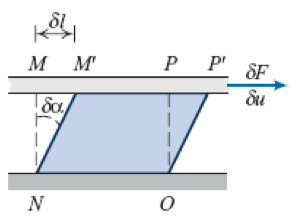
\includegraphics[width=.6\linewidth]{imgs/tens_cisa.png}
                    \caption{Modelagem da Tensão de Cisalhamento}
                \end{subfigure}% Really important to have this comment here and no black line
            \begin{subfigure}{.5\textwidth}
                \centering
                    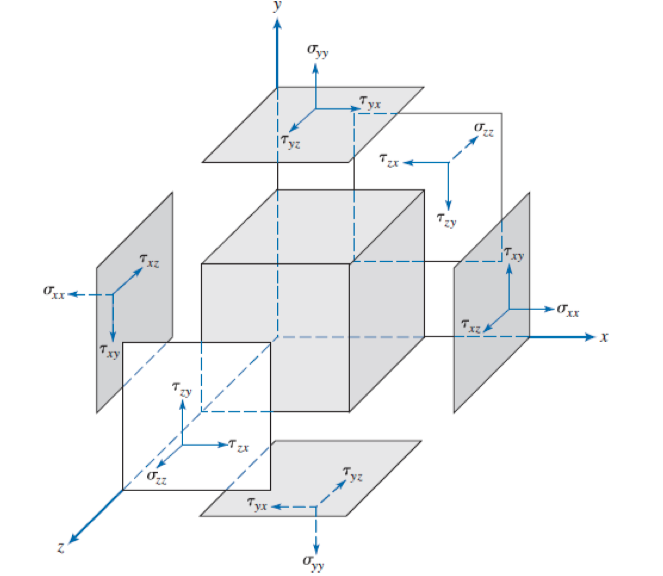
\includegraphics[width=.6\linewidth]{imgs/conv_tens.png}
                    \caption{Convenção de Sinais de Tensão}
                \end{subfigure}
            \end{figure}



        \end{table}
            



            


    
\end{document}